%%%%%%%%%%%%%%%%%%%%%%%%%%  example_onecolumn.tex  %%%%%%%%%%%%%%%%%%%%%%%%%%%%%%%%
%
% This is example_onecolumn.tex, an example file for use with the SIAM LaTeX2E
% Proceedings macros. It is designed to provide single-column output. Please 
% take the time to read the following comments, as they document how to use the
% SIAM Proceedings macro files. This file can be composed and printed out for
% use as sample output.
%
% Please submit suggestions for changes to: tex@siam.org.
%
% This file is to be used as an example for style only. It should not be read
% for content.

%%%%%%%%%%%%%%% PLEASE NOTE THE FOLLOWING STYLE RESTRICTIONS %%%%%%%%%%%%%%%

%%  1. There are no new tags.  Existing LaTeX tags have been formatted to match
%%     the SIAM Proceedings style.
%%
%%  2. Do not change the margins or page size!  Do not change from the default
%%     text font or the default text size of 10pt!
%%
%%  3. We recommend that you use BibTeX and siamplain.bst to list your references.
%%     You can use \cite in the text to mark your reference citations and
%%     \bibitem in the listing of references at the end of your chapter. See
%%     the examples in the following file. If you do use BibTeX, please supply
%%     your bib or bbl file with the manuscript file.
%%
%%  4. This macro is set up for two levels of headings (\section and
%%     \subsection). The macro will automatically number the headings for you.
%%
%%  5. No running heads are to be used.
%%
%%  6. Theorems, Lemmas, Definitions, Equations, etc. are to be double numbered,
%%     indicating the section and the occurrence of that element within that 
%%     section. (For example, the first theorem in the second section would be 
%%     numbered 2.1. The macro will automatically do the numbering for you.
%%
%%  7. Figures and Tables must be single-numbered. Use existing LaTeX tags for 
%%     these elements. Numbering will be done automatically.
%%
%%  8. Page numbering is not included in this macro since pagination
%%     will be set by the program committee.
%%

\documentclass[twoside,leqno]{article}

% Comment out the line below if using A4 paper size
\usepackage[letterpaper]{geometry}

\usepackage{siamproceedings}

\usepackage[T1]{fontenc}
\usepackage{amsmath,amssymb,amsfonts}
\usepackage{graphicx}
\usepackage{epstopdf}
\usepackage{enumitem}
%\usepackage{algorithmic}

\usepackage[title]{appendix}
\usepackage{listings}
\usepackage{algorithm}
\usepackage{algorithmicx}
\usepackage{algpseudocode}
\usepackage{tikz}
\usepackage{url}
\usepackage{adjustbox}
\usepackage{textcomp}
\usepackage{hyperref}
\usepackage{tcolorbox}
%\usepackage{apxproof}
\usetikzlibrary{arrows.meta,backgrounds}
\usetikzlibrary{arrows,automata}
\usetikzlibrary{arrows.meta,positioning,decorations.pathreplacing}
%\newtheorem{theorem}{Theorem}

\lstset{
    basicstyle=\ttfamily,
    breaklines=true,
    frame=single,
    language=HTML,
    showstringspaces=false,
    commentstyle=\color{gray},
    keywordstyle=\color{blue},
    stringstyle=\color{red},
    upquote=true
}

\newtcolorbox{stoppingcondition}[1][]{
  colback=cyan!10!white,
  colframe=cyan!75!black,
  fonttitle=\bfseries\large,
  title=#1,
  boxrule=1.5pt,
  left=12pt,
  right=12pt,
  top=10pt,
  bottom=10pt
}

%% ---- orbit colours (same pastel family as the unfolding figure) ----
\tikzset{
  vtx/.style   ={circle,draw=black!70,line width=0.5pt,minimum size=7mm,
                 inner sep=0pt,font=\small},
  orbA/.style  ={vtx,fill=blue!12},
  orbB/.style  ={vtx,fill=orange!20},
  orbC/.style  ={vtx,fill=green!16},
  orbD/.style  ={vtx,fill=violet!16},
  orbE/.style  ={vtx,fill=yellow!35},
  ed/.style    ={->,draw=black!70,line width=0.6pt},
  edbreak/.style ={->,draw=red!65!black,line width=0.9pt},
  ann/.style     ={font=\footnotesize,inner sep=1.5pt},
}


\ifpdf
  \DeclareGraphicsExtensions{.eps,.pdf,.png,.jpg}
\else
  \DeclareGraphicsExtensions{.eps}
\fi

% Add a serial/Oxford comma by default.
\newcommand{\creflastconjunction}{, and~}

% Used for creating new theorem and remark environments
\newsiamremark{remark}{Remark}
\newsiamremark{hypothesis}{Hypothesis}
\crefname{hypothesis}{Hypothesis}{Hypotheses}
\newsiamthm{claim}{Claim}

%%Currently, the algorithm title font matches the figure and table title
%%fonts. To make the algorithm title font appear as small caps, uncomment
%%the following code:

%\makeatletter
%\renewcommand{\ALG@name}{\sc Algorithm}
%\makeatother

\usepackage{amsopn}
\DeclareMathOperator{\diag}{diag}


\begin{document}

%
\newcommand\relatedversion{}
%\renewcommand\relatedversion{\thanks{The full version of the paper can be accessed at \protect\url{https://arxiv.org/abs/0000.00000}}} % Replace URL with link to full paper or comment out this line

\title{\Large Directed Graph Hashing\relatedversion}
    \author{Caleb Helbling\thanks{Draper (\email{chelbling@draper.com}).}}

\date{}

\maketitle

% Copyright Statement
% When submitting your final paper to a SIAM proceedings, it is requested that you include
% the appropriate copyright in the footer of the paper.  The copyright added should be
% consistent with the copyright selected on the copyright form submitted with the paper.
% Please note that "20XX" should be changed to the year of the meeting.

% Default Copyright Statement
\fancyfoot[R]{\scriptsize{Copyright \textcopyright\ 20XX by SIAM\\
Unauthorized reproduction of this article is prohibited}}

% Depending on which copyright you agree to when you sign the copyright form, the copyright
% can be changed to one of the following after commenting out the default copyright statement
% above.

%\fancyfoot[R]{\scriptsize{Copyright \textcopyright\ 20XX\\
%Copyright for this paper is retained by authors}}

%\fancyfoot[R]{\scriptsize{Copyright \textcopyright\ 20XX\\
%Copyright retained by principal author's organization}}

%\pagenumbering{arabic}
%\setcounter{page}{1}%Leave this line commented out.

\begin{abstract}
  In this paper we present various methodologies and algorithmic implementations for hashing node-labeled directed graphs. We distinguish between hashing graphs based on their global structure and hashing based on local observerations obtained by traversing the graph. Our approaches are careful to take into account any symmetry in the graph, so that nodes that are identical modulo automorphism or unfolding are assigned equal hashes. Structurally hashing trees has seen widespread use in blockchain, source code version control, and web applications. Despite the popularity of tree hashing, directed graph hashing remains unstudied in the literature.
\end{abstract}

\section{Introduction}\label{sec:introduction}

Hashing functions are fundamental building blocks in the modern software stack that have seen widespread use in data storage and retrieval, digital fingerprinting, checksum and cryptographic applications. Traditionally, hash functions take as input bit strings of arbitrary length and return a bit string of a fixed size $\mathcal{H} : \{0,1\}^* \rightarrow \{0,1\}^n$. Good hashing functions should be fast to compute, minimize the chance of duplication of output values, and produce large changes in output for small changes in input. Many bit string hashing functions have been created over the years, such as MD5 \cite{md5}, SHA-2 \cite{sha2}, and SHA-3 \cite{sha3}.

\begin{algorithm}
\caption{Recursive Merkle-tree Hashing of Ordered Binary Tree}
\[
\text{mh}(n) =
\begin{cases} 
    \mathcal{H}(n.\text{label}) & n \text{ is a leaf} \\
    \mathcal{H}(n.\text{label} \circ \text{mh}(n.\text{left}) \circ \text{mh}(n.\text{right})) & \text{otherwise}
\end{cases}
\]
\label{alg:merklehashing}
\end{algorithm}

Hashing functions can be extended to trees via a simple extension of Merkle hashing \cite{merkle1987digital}. In Merkle tree hashing, the hash of a node is computed by hashing the concatenation of the node's label with the recursive hash of the node's children. Algorithm \ref{alg:merklehashing} gives a simple recursive implementation of Merkle tree hashing for ordered binary trees. This particular variation of Merkle hashing has seen use in many applications, including cryptocurrency \cite{bitcoin}, version control systems \cite{git}, and distributed hypertext document storage systems \cite{ipfs}.

Extending hashing to node-labeled directed graphs is non-trivial due to the presence of cycles. Indeed, the design space of algorithm design for hashing digraphs is surprisingly broad and depends on use case objectives. In this paper we will focus on the following approaches, which we think are the most useful for practical applications:

\begin{itemize}
  \item \textbf{Global Hashing} (Section \ref{sec:global-graph-hashing}) - for use cases where the \textit{global} structure of the digraph is of importance. A correct algorithm should produce equal hashes if and only if two graphs are isomorphic. Nodes in the graph should hash to the same value if and only if them come from isomorphic graphs and they are identical modulo automorphism.
  \item \textbf{Local Hashing} (Section \ref{sec:local-graph-hashing}) - for use cases where observers can only observe \textit{local} information by traversing from a node to a neighbor on an outgoing edge. There are several formulations of local hashing, but in this paper we will discuss an algorithm that produces equal hashes for nodes if and only if the (potentially infinite) unfoldings from outward exploration are isomorphic. Local hashing has many commonalities with bisimulation and co-inductive representations of finite directed graphs \cite{bisimulation_book,coinductive_graphs}.
  \item \textbf{Ordered Outgoing Edges} (Section \ref{sec:outgoing-ordered-edge-graphs}) - in many practical applications the outgoing edges from a node are ordered. We can use this additional structure to simplify and improve the runtime performance of our hashing algorithms.
  \item \textbf{Merkle Graph Hashing} (Section \ref{sec:merkle-graph-hashing}) - for use cases where we want graphs to be hashed recursively, or graphs are structures that are built up over time. In this approach we hash strongly connected components individually using either global or local hashing, then recurse over the acyclic condensation graph induced by the strongly connected components.
\end{itemize}

One common theme throughout this paper is reliance on conversion of graphs to \textit{canonical form}. If two graphs (or nodes within) can be converted to a canonical form, we can serialize the canonical form and pass it through an ordinary string function.

We should additionally take care to distinguish between the hash of an entire graph vs the hash of a specific node within a graph. Our general strategy for computing the hash of a specific node is to combine the overall graph hash with the node's position in canonical order. Care must be taken to ensure that our index accounts for any symmetry present in the graph (ie, two nodes may be identical modulo automorphism).

%As we will see in the remainder of this paper, extending hashing to directed graphs gives a suprisingly broad range of options in algorithm design. To illustrate the design space, consider the case of hashing molecular structures (in the chemistry sense) for an informational database. In this case, the hash of the molecular directed graph depends on the \textit{global} structure of the digraph, and a correct algorithm should produce equal hashes if and only if two graphs are isomorphic.

%As a second example, consider the use case of a content-address web browser application that retrieves pages from a distributed hash table. In this case, the hash of a particular page in the web graph should only depend on the \textit{local} observations that can be made on a particular page and in the transitive closure. In other words, the hash of two web pages should be equal if and only if it is impossible to observationally distinguish between the two by navigating the web graph. This formulation of the graph hashing problem is directly related to the concept of bisimulation and coinductive representations of directed graphs.

%In this paper we will explore the extremes of this design space. For hashing digraphs in a global sense, we will make use of graph canonization algorithms and vertex orbit partitioning. We will then extend this approach to create a recursive variant that recurses over the acyclic condensation graph. We will then examine the other extreme by investigating \textit{directed vertex languages}, a variation of formal languages similar to finite automata. Unless otherwise stated, the graphs we are examining in this paper are node labeled directed graphs where nodes with duplicate labels are allowed.


%Hashing directed graphs adds an additional layer of complexity not present in trees. Directed graphs can have arbitrary cycles, which prevents the use of na\"ive recursion. We work around this issue via two different prongs. First, we make use of graph canonization algorithms, which can be used to give a unique order to the nodes. This order can be used to output an adjacency list, which can then be hashed with an ordinary string hashing function. Second, we use the structure of the graph condensation, which is an induced directed acyclic graph and therefore amenable to recursion.

%Our contributions in this paper can therefore be described as follows:

%\begin{itemize}
%    \item We give an algorithm for hashing an entire directed graph using graph canonization.
%    \item We give an algorithm for hashing specific nodes within a digraph. This approach takes into account any symmetry present within the graph.
%    \item We give quadratic time algorithms for hashing based on depth-first search in the special case where outgoing node edges are strictly ordered.
%    \item We outline a recursive approach for hashing cyclic directed graphs, drawing inspiration from Merkle-tree hashing. Although this approach cannot be used to fingerprint graphs in a global sense, we will make a bisimulation argument from the perspective of an observer traversing a graph that this approach is sufficient for many use cases.
%\end{itemize}

\section{Background}

\begin{figure*}[!b]
\centering
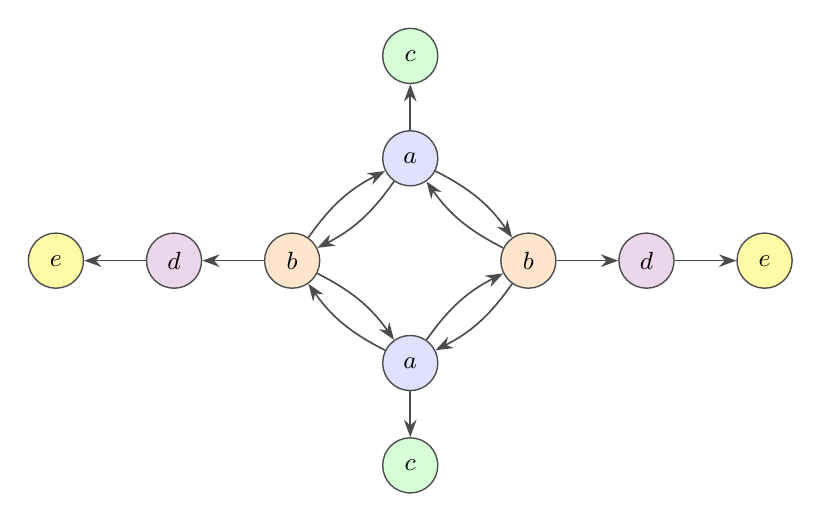
\begin{tikzpicture}[
  >={Stealth[length=2.2mm,width=1.6mm]},
  x=1cm, y=1cm,
]

%% ---------------- vertices ----------------
%% the layout is invariant under a 180-degree rotation about the centre,
%% which is exactly the symmetry that induces the orbits
\node[orbC] (e) at ( 0.0, 2.6) {$c$};
\node[orbA] (a) at ( 0.0, 1.3) {$a$};
\node[orbB] (b) at (-1.5, 0.0) {$b$};
\node[orbB] (c) at ( 1.5, 0.0) {$b$};
\node[orbA] (d) at ( 0.0,-1.3) {$a$};
\node[orbC] (f) at ( 0.0,-2.6) {$c$};

\node[orbD] (g) at ( 3.0, 0.0) {$d$};
\node[orbE] (h) at ( 4.5, 0.0) {$e$};
\node[orbD] (i) at (-3.0, 0.0) {$d$};
\node[orbE] (j) at (-4.5, 0.0) {$e$};

%% ---------------- edges ----------------
%% bidirectional edges of the central diamond: one arc per direction
\foreach \u/\v in {a/b, a/c, b/d, c/d}{
  \draw[ed] (\u) to[bend left=14] (\v);
  \draw[ed] (\v) to[bend left=14] (\u);
}

%% pendant edges
\draw[ed] (a) -- (e);
\draw[ed] (d) -- (f);
\draw[ed] (c) -- (g);
\draw[ed] (g) -- (h);
\draw[ed] (b) -- (i);
\draw[ed] (i) -- (j);

\end{tikzpicture}
\caption{This directed graph contains five orbits, identified by the letters
$a$, $b$, $c$, $d$ and $e$ and by the node colours. Nodes within the same
orbit are structurally identical due to the symmetry of the directed graph:
the drawing is invariant under a rotation by $180^\circ$, which maps every
node onto its orbit partner.}
\label{fig:orbitexample}
\end{figure*}

We now give some brief graph theory definitions required for this paper, which a more general audience interested in hashing may not be informed about.

An \textit{automorphism} of some graph $G=(V,E,L)$ is defined as a permutation $\sigma$ of vertices such that $(u, v) \in E$ if and only if $(\sigma(u), \sigma(v)) \in E$. Here $L$ is a labeling function that maps vertices to strings. Informally, the automorphism group gives all of the ways that $G$ is symmetrical.

\[
\text{Aut}(G) = \{ \sigma : V \rightarrow V \mid (u, v) \in E \leftrightarrow (\sigma(u), \sigma(v)) \in E\}
\]

A \textit{vertex orbit} is the equivalence class of vertices of a graph under the action of automorphisms. Informally, the orbit of a vertex $v$ can be thought of as the set of vertices that are symmetrically identical to $v$. Figure \ref{fig:orbitexample} gives an example of how orbits can be used to partition a graph.

\[
\text{Orb}(G, v) = \{u \in V \mid \exists \sigma \in \text{Aut}(G) \text{ such that } \sigma(v) = u\}
\]

\textit{Canonical labeling} is the process of ordering graph vertices such that isomorphic graphs canonize to the same value. Note that canonical labeling algorithms cannot distinguish between different graph automorphisms. Algorithms that can compute canonical labels are widely used in practice for graph isomorphism testing. Some examples of canonical labeling algorithms include nauty \cite{nauty}, bliss \cite{bliss}, and saucy \cite{saucy}.

\begin{figure}
  \centering
  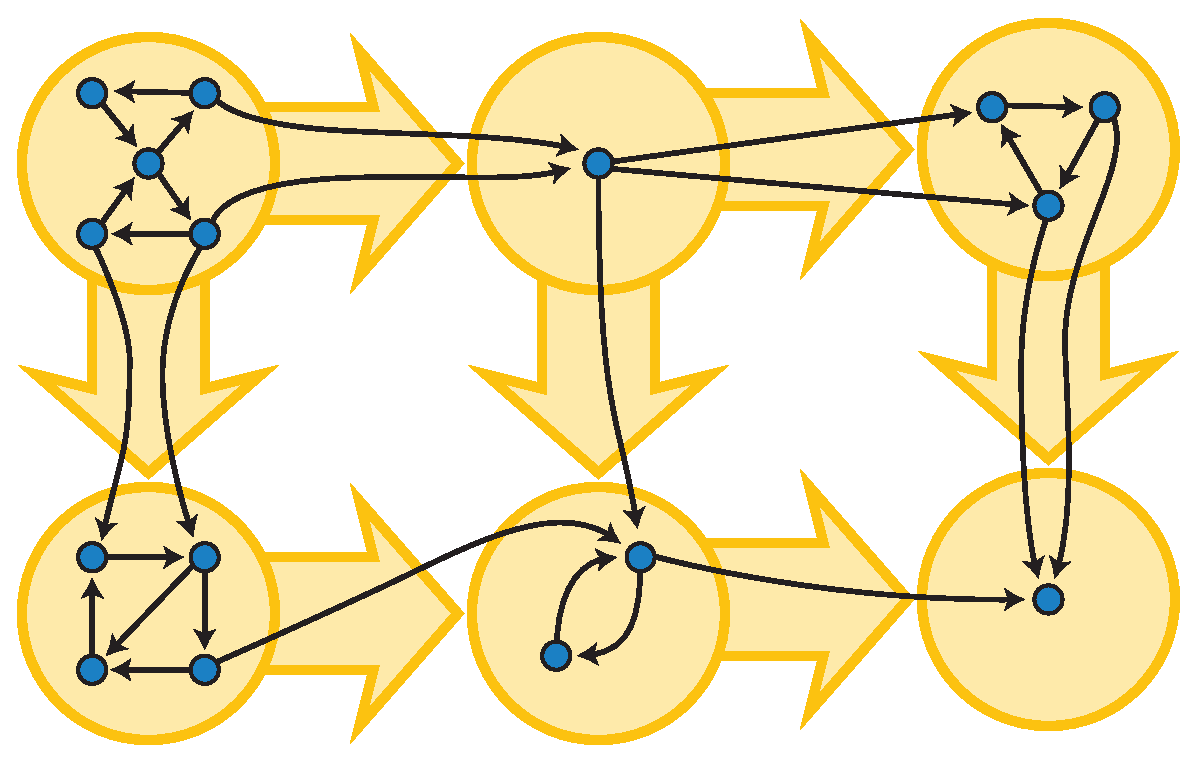
\includegraphics[width=0.5\linewidth]{Fig2.eps}
  \caption{Each yellow node contains a strongly connected component of a graph. When each strongly connected component is contracted into a single node, the yellow condensation graph is formed. Since the condensation graph is acyclic, it can be recursed over. Public domain figure courtesy of David Eppstein.\protect\footnotemark}
  \label{fig:condensation}
\end{figure}

The recursive Merkle-style algorithm will utilize the analysis of cycles within a directed graph. A \textit{strongly connected component} of a graph is a maximal set of vertices such that there exists a path in the graph between any two vertices within the strongly connected component. A \textit{condensation graph} is formed by contracting strongly connected components into single nodes. We will exploit the acyclicity of the condensation graph to construct our Merkle-style recursive algorithm. Figure \ref{fig:condensation} shows an example of strongly connected components and the induced condensation graph.

\section{Global Graph Hashing}
\label{sec:global-graph-hashing}

\footnotetext{\url{https://commons.wikimedia.org/wiki/File:Graph_Condensation.svg}}

\begin{algorithm}[b]
    \caption{Global Digraph Hash}\label{digraphhash}
    \begin{algorithmic}[1]
    \Function{$\mathcal{H_G}$}{$G=(V,E,L)$}
        \State \Comment{V is the set of vertices, E is the set of edges, L is the node labeling function}
        \State $\rho \gets$ \textproc{canonize}($G$) \Comment{\textproc{canonize} returns a mapping from vertices to their location in the canonical order}
        \State adj\_list $\gets$ \textproc{sort}($[(\rho(u), \rho(v)) \mid (u,v) \in E]$)
        \State labels $\gets$ [L($\rho^{-1}(n)$) \textbf{for} n \textbf{in} 0..\textbar V\textbar]
        \State \Return $\mathcal{H}$(\textproc{to\_str}((labels, adj\_list))) \Comment{Here $\mathcal{H}$ is a string hashing function such as SHA-3}
    \EndFunction
    \end{algorithmic}
\end{algorithm}

In global graph hashing, we would like our computed hash values to be unique modulo graph isomorphism. To be more precise, the hash of a graph $\mathcal{H_G}$ has the property $\mathcal{H_G}(G_1)=\mathcal{H_G}(G_2)$ if and only if $G_1 \cong G_2$. To achieve this correctness properties, we build on top of the well known string hashing functions and canonical labeling algorithms. We begin by canonizing the input digraph and constructing an adjacency list sorted in canonical order. The node labels (in canonical order) and the canonized adjacency list are then encoded as strings and hashed using a string hashing function $\mathcal{H}$. Algorithm \ref{digraphhash} gives an implementation of this approach.

Note that since we use generic graph canonization and orbit detection algorithms, our approach does not run in polynomial time. Indeed, graph hashing can trivially be use used to decide graph isomorphism, and as a consequence is \textbf{GI-Hard}. Since graph isomorphism is not thought to have a polynomial time algorithm, this means graph hashing likely does not have a polynomial time implementation.

%\begin{theorem}[Proof of Correctness]
\begin{theorem}[Global Hash Proof of Correctness]
\label{thm:digraphhashcorrect}
Assuming that the string hashing function $\mathcal{H}$ is injective, $\mathcal{H_G}(G_1)=\mathcal{H_G}(G_2)$ if and only if $G_1 \cong G_2$.
%\end{theorem}
\end{theorem}

\begin{proof}
($\Rightarrow$)If $\mathcal{H_G}(G_1)=\mathcal{H_G}(G_2)$, then the canonized adjacency list/vertex label lists are identical. If these representations of $G_1$ and $G_2$ are identical, then $G_1$ and $G_2$ have identical canonical form $G_3$. This means that $G_1 \cong G_3$ and $G_2 \cong G_3$, which implies that $G_1 \cong G_2$ by transitivity.

%Of course real string hashing functions are not injective by the pigeonhole principle, however in practice nobody has yet found collisions for algorithms such as SHA512. Therefore for this approach we treat string hashing algorithms as injective. The identity function or an asymmetric encryption algorithm are examples of truly injective string transformation functions, so those could be used as alternatives if desired.

($\Leftarrow)$ Let $G_3$ be the output graph of canonizing $G_1$, and $G_4$ be the output of canonizing graph $G_2$. Since $G_1 \cong G_2$, we conclude that $G_3=G_4$ since isomorphic graphs canonize to the same graph. This implies that the sorted adjacency lists and ordered vertex label lists are equivalent, so the string representation is equivalent. Therefore the string hash output are equivalent as well, which shows that $\mathcal{H_G}(G_1)=\mathcal{H_G}(G_2)$. 
\end{proof}

%\begin{inlineproof}
%Available in appendix
%\end{inlineproof}

\begin{algorithm}[t]
    \caption{Global Digraph Node Hash}\label{alg:digraph-node-hash}
    \begin{algorithmic}[1]
    \Function{$\mathcal{H_N}$}{$G$, $v$}
        \State $\rho \gets$ \textproc{canonize}($G$)
        \State g\_hash $\gets \mathcal{H_G}($G$)$
        \State orbit\_idx $\gets$ $\min(\text{Orb}(\rho(G), \rho(v)))$
        \State \Return $\mathcal{H}$(\textproc{to\_str}((orbit\_idx, g\_hash)))
    \EndFunction
    \end{algorithmic}
\end{algorithm}

The algorithm for hashing nodes in a graph builds on the algorithm for hashing graphs. First, the graph is canonized and the hash of the entire canonical graph is computed using Algorithm \ref{digraphhash}. Then we compute the orbit index of the input vertex, which is defined to be the canonical index of the equivalence class representative element, where the equivalence relation in this case is the vertex orbit. The orbit index and the graph hash are then combined and passed through a string hashing function. Algorithm \ref{alg:digraph-node-hash} gives an implementation of this approach.

\begin{theorem}[Global Node Hash Proof of Correctness]
\label{thm:digraphnodehashcorrect}
Nodes should hash to the same value if and only if they come from isomoprhic graphs and they are identical modulo vertex orbits. To be precise, $\mathcal{H_N}(v_1, G_1)=\mathcal{H_N}(v_2, G_2)$ if and only if $G_1 \cong G_2$, $\exists \phi . v_2 \in \text{Orb}(\phi(v_1), G_2)$, and $\exists \phi . v_1 \in \text{Orb}(\phi^{-1}(v_2), G_1)$ where $\phi : V_1 \rightarrow V_2$ is an isomorphism between $G_1$ and $G_2$.
\end{theorem}

\begin{proof}
($\Rightarrow$) If $\mathcal{H_N}(v_1, G_1)=\mathcal{H_N}(v_2, G_2)$, then the orbit index of $v_1$ in $\mathcal{H_N}(v_1, G_1)$ is equal to the orbit index of $v_2$ in $\mathcal{H_N}(v_2, G_2)$, and $\mathcal{H_G}(G_1)=\mathcal{H_G}(G_2)$ by the injectivity of string hashing. Then by Theorem \ref{thm:digraphhashcorrect}, $G_1 \cong G_2$.

Let $\rho_1$ be the canonization of $G_1$ and $\rho_2$ be the canonization of $G_2$. Then $\rho_1(G_1)=\rho_2(G_2)$ since $G_1 \cong G_2$. Note that $\rho_1$ and $\rho_2$ are both isomorphisms. Then let $\phi=\rho_2^{-1} \circ \rho_1$ and $\phi^{-1}=\rho_1^{-1} \circ \rho_2$. Applying this definition of $\phi$, we wish to show that $v_2 \in \text{Orb}(\rho_2^{-1}(\rho_1 (v_1)), G_2)$ and $v_1 \in \text{Orb}(\rho_1^{-1}(\rho_2 (v_2)), G_1)$. Applying the isomorphisms $\rho_2$ and $\rho_1$ to these sets respectively, this is equivalent to showing that $\rho_2(v_2) \in \text{Orb}(\rho_1 (v_1), \rho_2(G_2))$ and $\rho_1(v_1) \in \text{Orb}(\rho_2 (v_2), \rho_1(G_1))$.

Recall that the orbit index of $v_1$ in $\mathcal{H_N}(v_1, G_1)$ is equal to the orbit index of $v_2$ in $\mathcal{H_N}(v_2, G_2)$. This implies that the two orbit sets are equal $\text{Orb}(\rho_1 (v_1), \rho_1(G_1))=\text{Orb}(\rho_2 (v_2), \rho_2(G_2))$ since they have equal representative elements. Then since $\rho_1(G_1)=\rho_2(G_2)$, $\text{Orb}(\rho_1 (v_1), \rho_1(G_1))=\text{Orb}(\rho_2 (v_2), \rho_2(G_2))=\text{Orb}(\rho_1 (v_1), \rho_2(G_2))$\\
$=\text{Orb}(\rho_2 (v_2), \rho_1(G_1))$. Then trivially $\rho_1(v_1) \in \text{Orb}(\rho_1 (v_1), \rho_1(G_1))$ and $\rho_2(v_2) \in \text{Orb}(\rho_2 (v_2), \rho_2(G_2))$. Following the chain of equalities and making the appropriate substitutions, then $\rho_2(v_2) \in \text{Orb}(\rho_1 (v_1), \rho_2(G_2))$ and $\rho_1(v_1) \in \text{Orb}(\rho_2 (v_2), \rho_1(G_1))$.

($\Leftarrow$) If $G_1 \cong G_2$, then $\mathcal{H_G}(G_1)=\mathcal{H_G}(G_2)$ by Theorem \ref{thm:digraphhashcorrect}. Then there exists some isomorphism $\phi$ and $\phi'$ such that $v_2 \in \text{Orb}(\phi(v_1),G_2)$ and $v_1 \in \text{Orb}(\phi'^{-1}(v_2),G_1)$. Let $\rho_1$ be the canonization of $G_1$ and $\rho_2$ be the canonization of $G_2$. Applying these isomorphisms, we have $\rho_2(v_2) \in \text{Orb}(\rho_2(\phi(v_1)), \rho_2(G_2))$ and $\rho_1(v_1) \in \text{Orb}(\rho_1(\phi'^{-1}(v_2)),\rho_1(G_1))$. Let $f=\rho_1 \circ \phi^{-1} \circ \rho_2^{-1}$ and $f'=\rho_2 \circ \phi' \circ \rho_1^{-1}$ be automorphisms over the canonized graph.

Then by definition of orbit, $\text{Orb}(\rho_2(\phi(v_1)), \rho_2(G_2))=\text{Orb}(f(\rho_2(\phi(v_1))), \rho_2(G_2))$ and $\text{Orb}(\rho_1(\phi'^{-1}(v_2)),\rho_1(G_1)) = \text{Orb}(f'(\rho_1(\phi'^{-1}(v_2)),\rho_1(G_1)))$. Substituting in the definitions of $f$ and $f'$, we have $\text{Orb}(\rho_2(\phi(v_1)), \rho_2(G_2))=\text{Orb}(\rho_1(v_1), \rho_2(G_2))$ and $\text{Orb}(\rho_1(\phi'^{-1}(v_2)),\rho_1(G_1)) = \text{Orb}(\rho_2(v_2),\rho_1(G_1))$. This shows that $\rho_2(v_2) \in \text{Orb}(\rho_1(v_1), \rho_2(G_2))$ and $\rho_1(v_1) \in \text{Orb}(\rho_2(v_2),\rho_1(G_1))$. Since $G_1 \cong G_2$, $\rho_1(G_1)=\rho_2(G_2)$ so $\rho_2(v_2) \in \text{Orb}(\rho_1(v_1), \rho_1(G_1))$ and $\rho_1(v_1) \in \text{Orb}(\rho_2(v_2),\rho_2(G_2))$. This suffices to show that the orbit indices of are equal in the computations of $\mathcal{H_N}(v_1, G_1)$ and $\mathcal{H_N}(v_2, G_2)$.

Since the orbit indices are equal and $\mathcal{H_G}(G_1)=\mathcal{H_G}(G_2)$, then $\mathcal{H_N}(v_1, G_1)=\mathcal{H_N}(v_2, G_2)$. 
\end{proof}

%\begin{inlineproof}
%Available in appendix
%\end{inlineproof}

\section{Local Graph Hashing}
\label{sec:local-graph-hashing}

\begin{figure}[htbp]
\centering
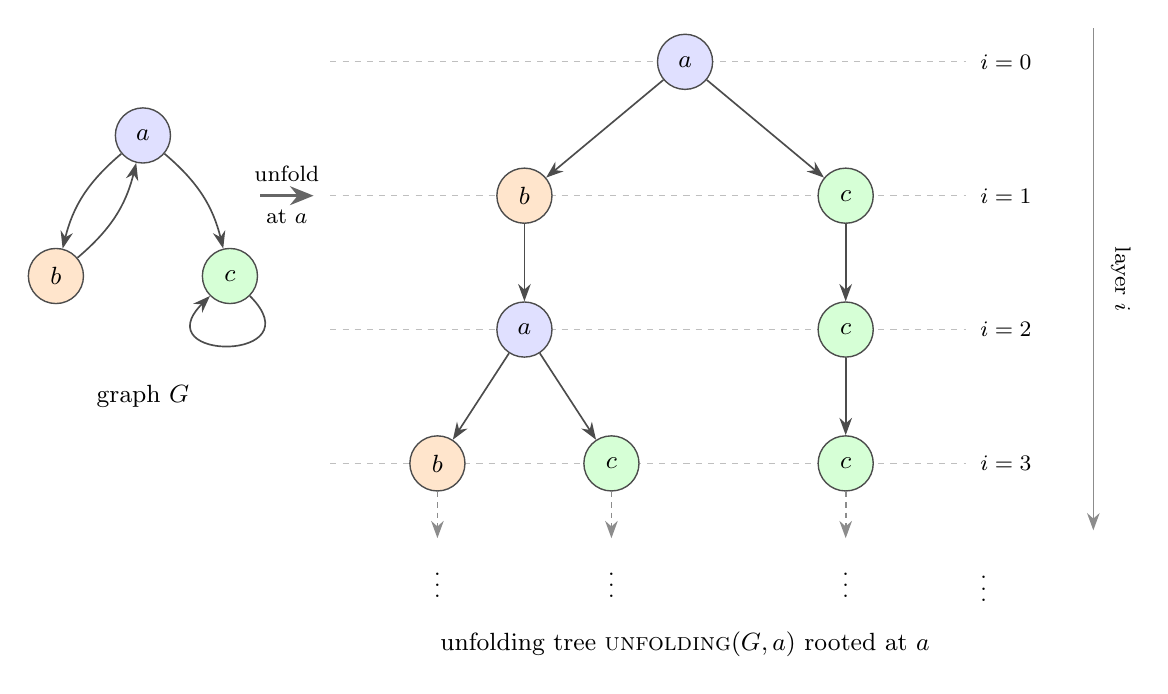
\begin{tikzpicture}[
  x=0.85cm, y=0.85cm,
  >={Stealth[length=2.2mm,width=1.6mm]},
  vtx/.style    ={circle,draw=black!70,line width=0.5pt,minimum size=7mm,
                  inner sep=0pt,font=\small},
  va/.style     ={vtx,fill=blue!12},
  vb/.style     ={vtx,fill=orange!20},
  vc/.style     ={vtx,fill=green!16},
  ed/.style     ={->,draw=black!70,line width=0.6pt},
  cont/.style   ={->,draw=black!45,line width=0.6pt,
                  dash pattern=on 2pt off 1.8pt,shorten >=2pt},
  layer/.style  ={draw=black!25,dash pattern=on 2.2pt off 2.2pt,line width=0.4pt},
  ilab/.style   ={font=\footnotesize,anchor=west,inner sep=2.5pt},
  dots/.style   ={font=\footnotesize,inner sep=1pt},
]
%% ------------------------------------------------------------------
%% layer guides (drawn first so that they sit behind the nodes)
%% ------------------------------------------------------------------
\foreach \y/\i in {0/0, -2/1, -4/2, -6/3}{%
  \draw[layer] (-5.3,\y) -- (4.2,\y);
  \node[ilab] at (4.3,\y) {$i=\i$};
}
\node[ilab] at (4.3,-7.75) {$\vdots$};
%% layer axis
\draw[->,draw=black!45,line width=0.5pt] (6.1,0.5) -- (6.1,-7.0)
      node[midway,right=1mm,font=\footnotesize,rotate=-90,anchor=south]
      {layer $i$};
%% ------------------------------------------------------------------
%% left: the graph G (with cycles)
%% ------------------------------------------------------------------
\begin{scope}[shift={(-8.1,-2.6)}]
  \node[va] (ga) at ( 0.0, 1.5) {$a$};
  \node[vb] (gb) at (-1.3,-0.6) {$b$};
  \node[vc] (gc) at ( 1.3,-0.6) {$c$};
  \draw[ed] (ga) to[bend right=18] (gb);   % a -> b
  \draw[ed] (gb) to[bend right=18] (ga);   % b -> a
  \draw[ed] (ga) to[bend left=18]  (gc);   % a -> c
  \draw[ed] (gc) to[out=-45,in=-135,looseness=6,
                    min distance=5mm] (gc);            % c -> c
  \node[font=\small] at (0,-2.4) {graph $G$};
\end{scope}
%% unfolding arrow
\draw[-{Stealth[length=3mm,width=2.4mm]},draw=black!60,line width=1pt]
      (-6.35,-2.0) -- (-5.55,-2.0)
      node[midway,above=0.5mm,font=\footnotesize]{unfold}
      node[midway,below=0.5mm,font=\footnotesize]{at $a$};
%% ------------------------------------------------------------------
%% right: the unfolding (infinite tree, finitely truncated)
%% ------------------------------------------------------------------
% i = 0
\node[va] (r)    at ( 0.0, 0) {$a$};
% i = 1
\node[vb] (b1)   at (-2.4,-2) {$b$};
\node[vc] (c1)   at ( 2.4,-2) {$c$};
% i = 2
\node[va] (a2)   at (-2.4,-4) {$a$};
\node[vc] (c2)   at ( 2.4,-4) {$c$};
% i = 3
\node[vb] (b3)   at (-3.7,-6) {$b$};
\node[vc] (c3)   at (-1.1,-6) {$c$};
\node[vc] (cc3)  at ( 2.4,-6) {$c$};
\draw[ed] (r)  -- (b1);
\draw[ed] (r)  -- (c1);
\draw[ed] (b1) -- (a2);
\draw[ed] (c1) -- (c2);
\draw[ed] (a2) -- (b3);
\draw[ed] (a2) -- (c3);
\draw[ed] (c2) -- (cc3);
% continuation of the infinite tree
\draw[cont] (b3)  -- (-3.7,-7.2);  \node[dots] at (-3.7,-7.7) {$\vdots$};
\draw[cont] (c3)  -- (-1.1,-7.2);  \node[dots] at (-1.1,-7.7) {$\vdots$};
\draw[cont] (cc3) -- ( 2.4,-7.2);  \node[dots] at ( 2.4,-7.7) {$\vdots$};
\node[font=\small] at (0,-8.7) {unfolding tree $\textproc{unfolding}(G, a)$ rooted at $a$};
\end{tikzpicture}
\caption{Unfolding of a directed graph with cycles. Starting from the root
$a$, every vertex is replaced by one copy per path reaching it, so the cycle
$a\to b\to a$ and the self-loop $c\to c$ are unrolled into an infinite tree;
only the layers $i=0,\dots,3$ are drawn. Each tree node at layer $i$
corresponds to a path of length $i$ from $a$ in $G$; colours indicate the
originating vertex of $G$. The color $\lambda_i(a)$ is equivalent to the hash
of the unfolding finite Merkle-tree up to layer $i$.}
\label{fig:unfolding}
\end{figure}

In comparison to the global hashing strategy which depends on the global structure of the graph, the local hashing strategy depends only on properties we can \textit{observe} by traversing the digraph forward along its edges. To make this concept precise, we say that the hash of two nodes in a digraph should be equal if and only if their \textit{unfoldings} are isomorphic. An unfolding is the formed by selecting a starting node, placing it at the root of the tree, then adding successor nodes as children, and expanding recursively. This forms a (potentially infinite) tree induced by the structure of the underlying digraph. Figure \ref{fig:unfolding} shows an example of an unfolding for a directed graph.

Our strategy for local graph hashing uses a variation of an algorithm to compute color refinement. In color refinement, nodes are repeatedly colored and propagated over multiple iterations until a stable coloring is achieved. To be more precise, the initial coloring $\lambda_0$ of the nodes is defined to be the hash of the node's labels:

\begin{equation}
  \lambda_0(u) = \mathcal{H}(L(u))
\end{equation}

We then compute colorings over multiple iterations using the following equation (note that $\{\{...\}\}$ is a multiset, and that a multiset can be converted to a string by sorting its members):

\begin{equation}
  \label{eq:coloring-step}
  \lambda_{i+1}(u) = \mathcal{H}(\textproc{to\_str}((L(u), \{\{\lambda_{i}(v) \mid (u, v) \in E\}\})))
\end{equation}

The color of a node in round $i$ is exactly the Merkle-hash of an unfolding tree with a maximum depth of $i+1$ layers. Note here that our unfolded finite tree is being built bottom-up, with a new layer added to the tree every iteration. Due to the bottom-up construction, the hashing process maximally shares computation, making this a dynamic programming approach.

We now define the following stabilization condition which will tell us when to stop computing new colors:

\begin{stoppingcondition}
\textbf{Global Stabilization Condition}: Global stabilization is achieved in round $i$ if for all nodes $u$, $v$ in $G$, $\lambda_{i+1}(u)=\lambda_{i+1}(v)$ if and only if $\lambda_i(u)=\lambda_i(v)$.
\end{stoppingcondition}

Our first step of local graph hashing, then, is to take the input graph and compute the stable colors of each node, stopping when the global stabilization condition is achieved. With this in hand, we then construct a quotient graph induced by the stable colors, merging any nodes together with identical color. Note here that the quotient graph produced is a multi-digraph, so that we preserve the unfolding of all nodes.

We then proceed to operate on the new quotient graph, and pass it through a fresh round of color refinement, this time making use of the following stabilization condition:

\begin{stoppingcondition}
\textbf{Local Stabilization Condition}: A node $n$ is locally stable in round $i$ if for all nodes $u$, $v$ in the reachable subgraph from $n$, $\lambda_{i+1}(u)=\lambda_{i+1}(v)$ if and only if $\lambda_i(u)=\lambda_i(v)$.
\end{stoppingcondition}

For each node $n$ in the quotient graph, there will be some step $i$ in which that node becomes locally stable. On that round we can create a canonical order for the nodes in the reachable subgraph of $n$ by sorting the colors $\lambda_i$ for each node. We can then use this ordering to create a canonical adjacency list, which can then be serialized to a string and passed through a string hashing function. This gives the node hash for vertex $n$.

\begin{algorithm*}[!b]
    \caption{Local Digraph Node Hash}\label{alg:local-node-hash}
    \begin{algorithmic}[1]

    \Function{\textproc{serialize}}{$Q=(V, E, L)$, root, reach, colors}
        \State order $\gets$ \textproc{sorted}(reach, key=colors)
        \State index $\gets$ $\{x \mapsto i \mid (i, x) \in \textproc{enumerate}(\text{order})\}$
        \State root\_idx $\gets$ index[root]
        \State adj\_list = \textproc{sorted}([(index[$s$], index[$t$] $\mid (s, t) \in E \land s \in \text{reach} \land t \in \text{reach}$)])
        \State labels $\gets$ [L(x) \textbf{for} $x$ \textbf{in} order]
        \State \Return $\mathcal{H}$(\textproc{to\_str}((root\_idx, labels, adj\_list)))
    \EndFunction

    \Function{$\mathcal{H_L}$}{$G=(V, E, L)$}
        \State $C \gets$ \textproc{global\_colors}($G$) \Comment Map nodes in $V$ to colors
        \State $Q \gets G / C$ \Comment Use colors as an equivalence class to compute a quotient multi-digraph
        \State $(V', E', L') \gets Q$ \Comment $L'$ maps nodes in $V'$ to the original node labels
        \State reach $\gets \{n \mapsto \textproc{reachable}(Q, n) \mid n \in V'\}$
        \State locally\_stable $\gets \{\}$
        \State final\_hash $\gets \textproc{empty\_dict}()$
        \State $\lambda \gets \{n \mapsto \mathcal{H}(L'(n)) \mid n \in V'\}$
        \While{$|\text{locally\_stable}|<|V'|$}
          \State $\lambda_{next} \gets$ \textproc{refine\_round}($Q, \lambda, L'$)
          \For{$n \in V'$}
            \If{$n \notin \text{locally\_stable}$}
              \If{\textproc{partition\_unchanged}(reach[n], $\lambda$, $\lambda_{next}$)}
                \State locally\_stable $\gets \text{locally\_stable} \cup \{n\}$
                \State final\_hash[n] $\gets$ \textproc{serialize}($Q$, $n$, reach[n], colors)
              \EndIf
            \EndIf
          \EndFor
          \State $\lambda \gets \lambda_{next}$
        \EndWhile
        \State \Return $\{n \mapsto \text{final\_hash}[C[n]] \mid n \in V\}$ \Comment Return the hashes for all nodes in the graph
    \EndFunction
    \end{algorithmic}
\end{algorithm*}

To summarize our approach, we begin by merging any nodes which are identical modulo tree expansion by using graph coloring with the global stabilization condition. We then construct a quotient graph, merging any of these identical nodes. We then compute a new graph coloring for each node, this time using the local stabilization condition. Since these colors are unique, they can be canonically ordered. The canonical ordering can then be used to construct a canonical adjacency list, which can then be hashed using an ordinary string hashing function. Algorithm \ref{alg:local-node-hash} gives a pseudo-code implementation of this approach that computes the hash for all nodes in the input graph.

We now show that the stabilization conditions (both global and local) are a sufficient stopping condition for the problem we are trying to solve:

\begin{lemma}
\label{thm:stability}
If stability (local or global) is achieved on round $i$, then the partition of colors (ie, by placing nodes with equal colors in the same partition) is unchanged for all future rounds $j > i$.
\end{lemma}
\begin{proof}
By induction on the round number. As a base case, consider $j=i+1$. By the definition of stable, the partition remains unchanged on this step. For the inductive step, assume in step $j$ the partition remains unchanged. When computing the colors for step $j+1$, the only value affecting the paritition of the nodes is the partition of the values from the previous step. In other words, the partition of the values in the multiset in Equation \ref{eq:coloring-step} remains the same. This means that the partition of the nodes remains unchanged in step $j+1$.
\end{proof}

By Lemma \ref{thm:stability}, we see that using the stable colors as an equivalence class when computing the quotient graph is the same as using the infinite limit of the colors (which is a Merkle-tree hash) as an equivalence class.

Our approach in this section draws inspiration from two different areas: classic color refinement algorithms that operate over \textit{undirected} graphs; also known as Weisfeiler-Lehman graph or subtree kernels \cite{Shervashidze2011-dt}, and DFA partition refinement strategies, such as Hopcraft's DFA minimization algorithm \cite{hopcraft, hopcraft-redescribe}. The idea of unfolding a graph into a tree for isomorphism testing has been discussed before in the literature on Weisfeiler-Lahman graph kernels \cite{Shervashidze2011-dt, fast_subtree_kernels_on_graphs}, however the locally stable condition and use of the colors as a canonical order for hashing is novel.

\begin{theorem}[Local Hash Proof of Correctness]
\label{thm:localhashcorrect}
Given some node $u$ from $G_1$ and some node $v$ from $G_2$, $\mathcal{H_L}(G_1)[u] = \mathcal{H_L}(G_2)[v]$ if and only if $\textproc{unfolding}(G_1, u) \cong \textproc{unfolding}(G_2, v)$
\end{theorem}

\begin{proof}
  ($\Rightarrow$) If $\mathcal{H_L}(G_1)[u] = \mathcal{H_L}(G_2)[v]$, then the reachable subgraphs in the quotient graph from $u$ and $v$ are identical. Since the unfolding depends only on the reachable parts of the graph, and taking the quotient leaves the unfolding unchanged, the unfoldings of the original graphs are isomorphic.

  ($\Leftarrow$) Let $V_1, E_1$ be the vertices and edges of the quotient graph $Q_1 = G_1 / C_1$ reachable from $u$. Let $V_2, E_2$ be the vertices and edges of the quotient graph $Q_2 = G_2 / C_2$ reachable from $v$.
  
  Then it is easy to construct a bijection $f$ of the vertices in the unfoldings since they are isomorphic. This bijection maps between nodes with isomorphic subtrees. Since the quotient graph merges any nodes with identical unfoldings, this same bijection can be re-interpreted as a bijective induced map $g : V_1 \rightarrow V_2$ between the nodes in the reachable portions of the quotient graphs.

  We now show that $g$ also preserves edges. That is, $(a, b) \in E_1$ if and only if $(g(a), g(b)) \in E_2$.
  
  Consider the following cases:
  \begin{itemize}
    \item If $(a, b) \in E_1$, then $(g(a), g(b)) \in E_2$. Assume that $(g(a), g(b)) \notin E_2$. Then $\textproc{unfolding}(G_1, a) \ncong  \textproc{unfolding}(G_2, g(a))$, which contradicts the assumption that the original bijection $f$ maps between isomorphic unfoldings.
    \item If $(g(a), g(b)) \in E_2$, then $(a, b) \in E_1$. Assume that $(a, b) \notin E_1$. Then $\textproc{unfolding}(G_1, a) \ncong  \textproc{unfolding}(G_2, g(a))$, which contradicts the assumption that the original bijection $f$ maps between isomorphic unfoldings.
  \end{itemize}

  We have therefore shown that the reachable portions of the quotient graph are isomorphic via $g$. We now note that the process of computing the final\_hash values in Algorithm \ref{alg:local-node-hash} is permutation invariant with respect to the quotient graph. This is because the color refinement portion of the computation is independent of vertex order, and the locally stable colors for each node when \textproc{partition\_unchanged} is true must be unique (by virtue of operating over a globally stable color quotient graph). We can therefore conclude that $\mathcal{H_L}(G_1)[u] = \mathcal{H_L}(G_2)[v]$. 
\end{proof}

%\begin{inlineproof}
%Available in appendix
%\end{inlineproof}

\subsection{Alternative Formulations of Local Hashing}

The strategy employed for local hashing depends on properties we can observe by traversing the graph forward along its directed edges. There are other formulations of local hashing, two of which we will note here:

\begin{enumerate}
  \item As a \textit{directed vertex language}. In this formulation, the hash of a node is defined as the hash of the (potentially infinite) set of strings that can be formed by visiting labeled nodes:
  
  \begin{equation}
  \text{Lang}_G(u) = \{L(u)\} \cup \bigcup_{v \in \text{successor}(u)} \{L(u) \circ x \mid x \in \text{Lang}_G(v)\}
  \end{equation}

  This particular formulation is very similar to that of nondeterminstic finite automata, except that characters are accumulated in a string by visiting nodes (instead of traversing edges), and all states can be terminal states. This formulation may be alternatively viewed as the set of walks that can be discovered by starting from a specific node.

  Our primary note on this formulation of local graph hashing is that computing a hash value of the set is \textbf{PSPACE-hard}. For this reason, we will not elaborate much further on solving this problem as an efficient algorithm is not possible.

  \textbf{Proof Sketch:} We perform a poly-time reduction from the NFA universality problem (UNIV), which is \textbf{PSPACE-complete} \cite{univ}. We say that an NFA is universal if it accepts every string. Given an input NFA, we can perform a poly-time version to an equivalent directed vertex language. We can then construct a universal NFA and encode it in a directed vertex language. If we could compute the hash of a directed vertex language, we could decide the equality between the input NFA and the universal NFA.

  \item As a \textit{bisimulation system}. The approach given in Section \ref{sec:local-graph-hashing} seeks to hash the unfolding, which is a slight twist on the philosophy of bisimulation. In a typical bisimulation setup, we say that nodes $a$ and $b$ are bisimilar if the following conditions are met:
  \begin{enumerate}
    \item $a$ and $b$ have the same label
    \item For every outgoing edge $a \rightarrow a'$, there exists a $b \rightarrow b'$ such that $a'$ and $b'$ are bisimilar.
    \item For every outgoing edge $b \rightarrow b'$, there exists a $a \rightarrow a'$ such that $b'$ and $a'$ are bisimilar.
  \end{enumerate}
  Note the use of the existential operator instead of a bijective mapping between successor nodes. This means that bisimulation inherently ignores duplicate bisimilar states. For example, two nodes may be bisimilar but have different out-degrees if multiple successor nodes are themselves bisimilar. Extending computation of a node's hash modulo bisimilarity instead of unfolding requires only a small modification to the previously described procedure: when computing the quotient graph $G/C$, collapse the graph to an ordinary digraph instead of a multi-digraph.
\end{enumerate}

\section{Outgoing Ordered Edge Graphs}
\label{sec:outgoing-ordered-edge-graphs}

\begin{figure*}[!b]
\centering
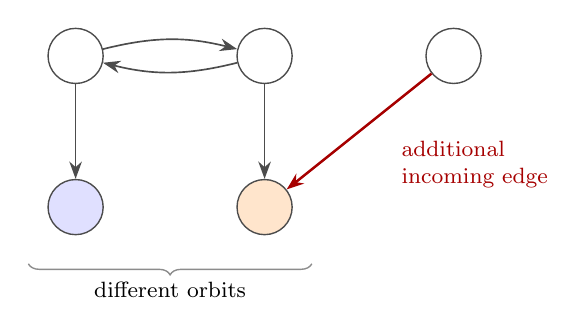
\begin{tikzpicture}[
  >={Stealth[length=2.2mm,width=1.6mm]},
  x=1.2cm, y=1.2cm,
]

%% ---------------- vertices ----------------
\node[vtx]  (a) at (0.0, 1.6) {};
\node[vtx]  (b) at (2.0, 1.6) {};
\node[vtx]  (e) at (4.0, 1.6) {};
\node[orbA] (c) at (0.0, 0.0) {};
\node[orbB] (d) at (2.0, 0.0) {};

%% ---------------- edges ----------------
\draw[ed] (a) to[bend left=14] (b);
\draw[ed] (b) to[bend left=14] (a);

\draw[ed] (a) -- (c);
\draw[ed] (b) -- (d);

%% the edge that destroys the candidate automorphism c <-> d
\draw[edbreak] (e) -- (d);
\node[ann,anchor=west,align=left,text=red!65!black] at (3.4,0.45)
      {additional\\incoming edge};

%% ---------------- annotation ----------------
\draw[decorate,decoration={brace,amplitude=4pt,mirror},draw=black!45,
      line width=0.5pt]
      (-0.5,-0.6) -- (2.5,-0.6)
      node[ann,midway,below=5pt] {different orbits};

\end{tikzpicture}
\caption{The symmetry of the two bottom nodes is broken by considering
incoming edges from higher in the graph. Without the highlighted edge the two
bottom nodes would be interchangeable; with it, no automorphism maps one onto
the other, so the two bottom nodes no longer lie in the same orbit.}
\label{fig:breaksymmetry}
\end{figure*}

For many real world applications of graph hashing, the labels of outgoing edges are strictly ordered.  We can take advantage of this extra structure on the edges to create simpler hashing algorithms. The algorithms in this section were directly inspired by the more general Scott graph canonization algorithm given by Bloyet, Marteau and Fr\'enod \cite{scott}. The basic idea for our approach is that due to the ordering of the edges, we can give an order to the nodes based on when they are visited in a graph traversal algorithm (in this case depth-first search).

%We can take advantage of this extra structure on the edges to create a node hashing algorithm that runs in polynomial time and neatly encapsulates the idea that the hash of a node should depend only the reachable subgraph structure. Algorithm \ref{alg:node-outgoing-edges} gives an overview of this approach based on the traversal order of a depth-first search. Note that the algorithms given in this section are directly inspired by the more general Scott graph canonization algorithm given by Bloyet, Marteau and Fr\'enod \cite{scott}.

\begin{algorithm}[H]
    \caption{Node Hash - Outgoing Ordered Edges}
    \label{alg:node-outgoing-edges}
    \begin{enumerate}
        \item For some input node $n$, perform a depth first search starting at $n$ and record the visitation order of the reachable nodes. Relabel each node in the order visited by the DFS.
        \item Create an adjacency list of this relabeled subgraph. Sort this adjacency list.
        \item Create a list of the original labels in the visitation order.
        \item Use a string hashing $\mathcal{H}$ on the (label list, adjacency list) tuple. This gives the hash of $n$.
    \end{enumerate}    
\end{algorithm}

For the \textbf{special case of a strongly connected graph}, we can use these hashes to compute both a canonical order and orbit partition in quadratic time. This special case is useful for the Merkle-style graph hashing algorithm given in Section \ref{sec:merkle-graph-hashing} where strongly connected components are hashed recursively.

\begin{algorithm}[H]
    \caption{Canonization and Orbit Partitioning for Strongly Connected Outgoing Ordered Edge Graphs}
    \label{alg:scc-outgoing-edges}
    \begin{enumerate}
        \item For each node $n$, compute the hash using Algorithm \ref{alg:node-outgoing-edges}. Nodes in the same orbit will have identical hash values, which can be used to compute the orbit partition. \textbf{Proof}: It is easy to construct an automorphism by examining the adjacency list constructed during the DFS.
        \item Take the node with the minimal hash value, and use its DFS ordering as the canonical order for the graph.
        \item At this point we now have a canonical order and orbit partition that can be used in Algorithm \ref{digraphhash} or \ref{alg:digraph-node-hash}.
    \end{enumerate}
\end{algorithm}

Why must we restrict ourselves to the special case of strongly connected graphs? In the case of a generic digraph, the symmetry and therefore the orbit of a node depends not only on the structure of the reachable subgraph, but also on the structure from ancestor nodes. Incoming edges from ancestor nodes can break the symmetry of an orbit, as demonstrated in Figure \ref{fig:breaksymmetry}. In the case of a strongly connected graph, this is not an issue as all nodes are mutual descendants.

\section{Merkle Graph Hashing}
\label{sec:merkle-graph-hashing}

For applications where graphs are built up over time taking a recursive algorithmic approach similar to Merkle-tree hashing would be highly beneficial. We will now construct such an algorithm that recursively operates over the condensation graph, which is a directed acyclic graph by construction. Algorithm \ref{alg:merklegraphhash} gives a pseudo-code implementation of the approach we will now discuss.

To compute the hash of a specific node, we begin by computing the strongly connected component containing the node. We then recursively compute the hashes of the targets of any edges leaving the strongly connected component. New labels for each node in the SCC are created by concatenating on the multiset of the hashes of non-SCC targets. Finally we compute the hash of each node using Algorithm \ref{alg:digraph-node-hash} (Algorithm \ref{alg:scc-outgoing-edges} can be used instead if the edges are ordered).

\begin{algorithm}
    \caption{Merkle Graph Node Hashing}\label{alg:merklegraphhash}
    \begin{algorithmic}[1]
    \Function{$\mathcal{H_M}$}{$G=(V,E,L), v$}
        \State $S \gets$ \textproc{Scc}($G, v$) \Comment{$S$ is the set of vertices in the strongly connected component containing $v$}
        \State $L'(x)=\mathcal{H}(\textproc{to\_str}((L(x),\{\{\mathcal{H_M}(G,y) \mid x \in S \land y \notin S \land (x,y) \in E\}\})))$ \\ \Comment{Relabel all nodes in the SCC using the recursively computed hashes of nodes outside the SCC}
        \State $(V', E', L'') \gets$ \textproc{Subgraph}($G, S$)
        \State $G' \gets (V',E',L')$
        \State \Return $\mathcal{H_N}(G', v)$ \Comment{Hash the relabelled SCC containing $v$ (Algorithm \ref{alg:scc-outgoing-edges} may be used instead if the outgoing edges are ordered)}
    \EndFunction
    \end{algorithmic}
\end{algorithm}

\section{Application Sketch}

\begin{figure}
\label{fig:webpage-example}
\centering

% Row 1: Original HTML snippets
\textbf{Row 1: Original HTML Pages}

\vspace{0.3cm}

\begin{adjustbox}{max width=\textwidth}
\begin{tabular}{p{5.5cm}@{\hspace{0.3cm}}p{5.5cm}@{\hspace{0.3cm}}p{5.5cm}}
index.html
\begin{lstlisting}[language=HTML]
<body>
 <h1>Welcome</h1>
 <a href="about.html">
  About Us
 </a>
 <a href="http://e.com">
  External Resource
 </a>
</body>
\end{lstlisting}
&
about.html
\begin{lstlisting}[language=HTML]
<body>
 <h1>About Us</h1>
 <a href="index.html">
  Home
 </a>
 <a href="contact.html">
  Contact
 </a>
 <a href="http://p.com">
  Partner Site
 </a>
</body>
\end{lstlisting}
&
contact.html
\begin{lstlisting}[language=HTML]
<body>
 <h1>Contact Us</h1>
 <a href="about.html">
  About
 </a>
 <a href="http://e.com">
  External Resource
 </a>
</body>
\end{lstlisting}
\end{tabular}
\end{adjustbox}

\vspace{0.5cm}

% Row 2: Tokenized/Hashed HTML snippets
\textbf{Row 2: Replace intra-SCC links with natural numbers in order of appearance, recursively hash inter-SCC links}

\vspace{0.3cm}

\begin{adjustbox}{max width=\textwidth}
\begin{tabular}{p{5.5cm}@{\hspace{0.3cm}}p{5.5cm}@{\hspace{0.3cm}}p{5.5cm}}
index.html
\begin{lstlisting}[language=HTML]
<body>
 <h1>Welcome</h1>
 <a href="{0}">
  About Us
 </a>
 <a href="#8ab43f">
  External Resource
 </a>
</body>
\end{lstlisting}
&
about.html
\begin{lstlisting}[language=HTML]
<body>
 <h1>About Us</h1>
 <a href="{0}">
  Home
 </a>
 <a href="{1}">
  Contact
 </a>
 <a href="#f2d91c">
  Partner Site
 </a>
</body>
\end{lstlisting}
&
contact.html
\begin{lstlisting}[language=HTML]
<body>
  <h1>Contact Us</h1>
  <a href="{0}">
    About
  </a>
  <a href="#8ab43f">
    External Resource
  </a>
</body>
\end{lstlisting}
\end{tabular}
\end{adjustbox}

\vspace{0.5cm}

% Row 3: Graph representation
\textbf{Row 3: Construct strongly connected directed graph (labels taken from previous row)}

\vspace{0.3cm}

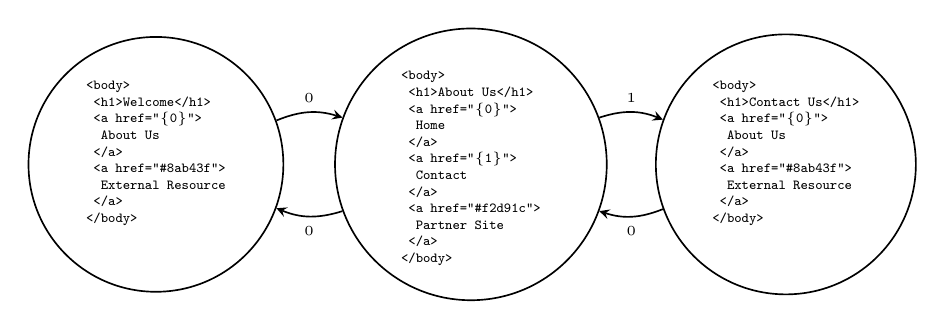
\begin{tikzpicture}[
    > = stealth, % arrow head style
    node distance=4cm,
    every node/.style={draw, align=left, font=\tiny},
    semithick % line style
]

% Nodes
\node[state] (index) {\\ \texttt{<body>} \\ \texttt{ <h1>Welcome</h1>} \\ \texttt{ <a href="\{0\}">} \\ \texttt{ ~About Us} \\ \texttt{ </a>} \\ \texttt{ <a href="\#8ab43f">} \\ \texttt{ ~External Resource} \\ \texttt{ </a>} \\ \texttt{</body>} \\ \\};
\node[state] (about) [right of=index] { \\ \texttt{<body>} \\ \texttt{ <h1>About Us</h1>} \\ \texttt{ <a href="\{0\}">} \\ \texttt{ ~Home} \\ \texttt{ </a>} \\ \texttt{ <a href="\{1\}">} \\ \texttt{ ~Contact} \\ \texttt{ </a>} \\ \texttt{ <a href="\#f2d91c">} \\ \texttt{ ~Partner Site} \\ \texttt{ </a>} \\ \texttt{</body>}};
\node[state] (contact) [right of= about] {\\ \texttt{<body>} \\ \texttt{ <h1>Contact Us</h1>} \\ \texttt{ <a href="\{0\}">} \\ \texttt{ ~About Us} \\ \texttt{ </a>} \\ \texttt{ <a href="\#8ab43f">} \\ \texttt{ ~External Resource} \\ \texttt{ </a>} \\ \texttt{</body>} \\ \\};

% Edges (internal links only)
\draw[->] (index) to[bend left=20] node[above, draw=none] {0} (about);
\draw[->] (about) to[bend left=20] node[below, draw=none] {0} (index);
\draw[->] (about) to[bend left=20] node[above, draw=none] {1} (contact);
\draw[->] (contact) to[bend left=20] node[below, draw=none] {0} (about);

\end{tikzpicture}

\caption{Visualization of procedure for hashing a three page HTML website. Note that in Row 2, the values \#8ab43f and \#f2d91c refer to hashes computed recursively - in this case the hash of pages on external websites.}

%Visualization of web page link structure: (Row 1) Original HTML with URLs, (Row 2) Tokenized version with internal links as \{n\} and external links as hash codes, (Row 3) Directed graph showing internal link structure with node labels corresponding to tokenized identifiers.}
\end{figure}

From the algorithms given so far, it may not be obvious how to implement these graph theoretic procedures for real world data. Here we will discuss how to do so by taking the example of a static hyperlinked web page system stored in a content addressed distributed hash table (DHT).

In this sketch, we will assume that our web pages are static HTML files which link to each other and to external websites. These files form a directed graph where each page is a node, and links between pages are edges. The outgoing edges from a node are labeled by natural numbers in the order in which the links appear in the HTML file. Figure \ref{fig:webpage-example} gives a concrete example of the process described here.

We begin by considering the links within each file and the strongly connected components created by our website. All intra-SCC links are replaced with natural numbers in the order in which the links appear. Links leaving the SCC are recursively hashed, and these hash values are inserted verbatim into the HTML of our webpages. We then compute the canonical order and orbit partition of the SCC in polynomial time using Algorithm \ref{alg:scc-outgoing-edges}. We then insert the following items into the distributed hash table:

\begin{itemize}
  \item The strongly connected component as a whole: \begin{itemize}
    \item \textbf{Value}: The canononically ordered adjacency list, along with the label list (ordered in the canonical order)
    \item \textbf{Key}: The string hash $\mathcal{H}$ of the value.
  \end{itemize}
  \item For each page, a reference to a specific node in the strongly connected component \begin{itemize}
    \item \textbf{Value}: The orbit index of the page, along with the overall SCC hash
    \item \textbf{Key}: The string hash $\mathcal{H}$ of the value.
  \end{itemize}
\end{itemize}

Suppose that a user wants to navigate our website, and has obtained a hash for one specific page. The browser software will begin by retrieving the orbit index and SCC hash from our distributed hash table (DHT). The browser then retrieves the SCC, giving us the adjacency list and allowing the SCC digraph to be reconstructed. The orbit index will then point us to a specific node in the SCC. The browser will display the contents of this node to the user.

If the user clicks a link within the same SCC, the browser simply follows the graph edge and shows the appropriate page contents. For links that leave the SCC, the browser repeats the same process from the beginning, retrieving the new SCC from the DHT.

\section{Related Work}

The core of the digraph Merkle hashing algorithm was independently discovered by the developers of the Unison programming language \cite{unison} for use in hashing abstract syntax trees of the Unison language. Each function and datatype in the Unison language is represented as a node in a digraph, with the AST acting as the node label. We note here that their approach does not take into account the possibility that nodes can lie in the same orbit, making their algorithm incomplete. In the real-world use of the Unison language, the possibility of non-singleton orbits is negligable, and could only occur in incredibly contrived situations.

The Weisfeiler-Lehman graph hash \cite{Shervashidze2011-dt} is a kernel method that iteratively hashes and aggregates neighborhoods of each node in an input graph. Isomorphic graphs are guaranteed to result in equal hashes, and a strong guarantee is given that non-isomorphic graphs will have different hashes. In the literature on this method an iteration parameter is often given as input, which leads to different outputs for different parameter settings. However this parameter is not actually necessary; termination is guaranteed to happen in $n-1$ rounds for a graph of size $n$ since the number of partitions can be at most $n$ and the number of partitions grows monotonically. The algorithm given in Section \ref{sec:local-graph-hashing} can be viewed as a type of Weisfeiler-Lehman graph hash.

In a 2014 paper, Arshad et al. \cite{Arshad2014-cc} presented an algorithm for hashing directed graphs, given additional inputs of a fixed source node and depth-first search traversal tree. The depth-first search traversal tree breaks the graph up into different edge types (tree, back, forward, and cross edges) depending on search order. The hashing algorithm then uses the traversal numbers to order the nodes and construct the hash. The authors note that isomorphic graphs may hash to different values due to this input dependence on source node and DFS tree. The approach presented by Arshad can be used to hash nodes with outgoing ordered edges, and can be viewed as an alternative to the algorithms presented in Section \ref{sec:outgoing-ordered-edge-graphs}.

In a separate 2018 paper, Arshad et al. \cite{Arshad2018-ij} presented a graph hashing algorithm where the hash of a node depends on the XORing together the hashes of the labels of all of that node's descendants. The hash of the entire graph is then computed by hashing each node concatenated with the accumulated graph hash. This approach is problematic in two different ways. While the node hash heuristic may be admissible in many cases, it is easy to construct two non-isomorphic graphs containing nodes with equal hashes, and therefore also equal graph hashes. Indeed, consider a $k$-clique and a $k$-cycle graph containing nodes with equivalent labels. These two graphs are not isomorphic, but each node has $k-1$ descendants, each of which are identically labelled. For this particular example, Arshad's algorithm will output equal hashes.

%Another problematic aspect of their approach lies with the dependence on DFS order. Two isomorphic graphs may have different graph hashes depending on the DFS order.

\section{Experimental Results}

% SIAM recommends using BibTeX
% if using BibTeX
\bibliographystyle{siamplain}
\bibliography{example_references}

\appendix

\end{document}

% else
%\begin{thebibliography}{10}
%
%\bibitem{Aggarwal06}
%{\sc G.~Aggarwal and J.~D. Hartline}, {\em Knapsack auctions}, in Proceedings
%  of the Seventeenth Annual ACM-SIAM Symposium on Discrete Algorithms (SODA),
%  Philadelphia, 2006, SIAM, pp.~1083--1092,
%  \url{http://dl.acm.org/citation.cfm?id=1109557.1109677}.
%
%\bibitem{amsmath}
%{\sc {American Mathematical Society}}, {\em User's guide for the
%  \texttt{amsmath} package (version 2.0)}, 2002,
%  \url{ftp://ftp.ams.org/pub/tex/doc/amsmath/amsldoc.pdf} (accessed
%  2015-07-30).
%
%\bibitem{Chew1989}
%{\sc L.~P. Chew}, {\em Guaranteed-quality triangular meshes}, Technical Report
%  89-983, Department of Computer Science, Cornell University, Apr. 1989.
%\newblock \url{https://hdl.handle.net/1813/6899}.
%
%\bibitem{CalcI}
%{\sc P.~Dawkins}, {\em Paul's online math notes: Calculus {I} --- notes},
%  \url{http://tutorial.math.lamar.edu/Classes/CalcI/MeanValueTheorem.aspx}
%  (accessed 2015-07-08).
%
%\bibitem{shortmath}
%{\sc M.~Downes}, {\em Short math guide for {\LaTeX}}, 2002,
%  \url{ftp://ftp.ams.org/pub/tex/doc/amsmath/short-math-guide.pdf} (accessed
%  2015-07-30).
%
%\bibitem{GoVa13}
%{\sc G.~H. Golub and C.~F. Van~Loan}, {\em Matrix Computations}, The Johns
%  Hopkins University Press, Baltimore, 4th~ed., 2013.
%
%\bibitem{MiGo04}
%{\sc F.~Mittlebach and M.~Goossens}, {\em The \LaTeX\ Companion},
%  Addison-Wesley, 2nd~ed., 2004.
%
%\bibitem{instance1290}
%{\sc B.~Stiller, T.~Bocek, F.~Hecht, G.~Machado, P.~Racz, and M.~Waldburger},
%  {\em Mobile systems {IV}}, tech. report, University of Zurich, Department of
%  Informatics, Jan. 2010.
%
%\bibitem{siam}
%{\em {SIAM} style manual: For journals and books}, 2013,
%  \url{https://epubs.siam.org/pb-assets/files/SIAM_STYLE_GUIDE_2019-1635349464967.pdf}.
%
%\end{thebibliography}
%
%\end{document}